In this section, we first outline our approximation-aware design strategies for optimizing \gls{ibc} performance (\gls{qoc}) and memory utilization. We determine what to approximate by identifying the error-resilient stages that can give maximum benefits on approximation (Section~\ref{profile}). Then, we explain how to approximate by summarizing the main steps of our approximation-aware \gls{ibc} design (Section~\ref{coarse_approx}). We then proceed to show how to interpret the outcomes by introducing a \gls{qoc}-optimal mode for approximated IBC systems (Section~\ref{analyze}). Finally, we describe the quality metrics considered for evaluation (Section~\ref{metrics}). 

% \vspace{-5 pt}
\begin{figure}[thb]
	\centering
	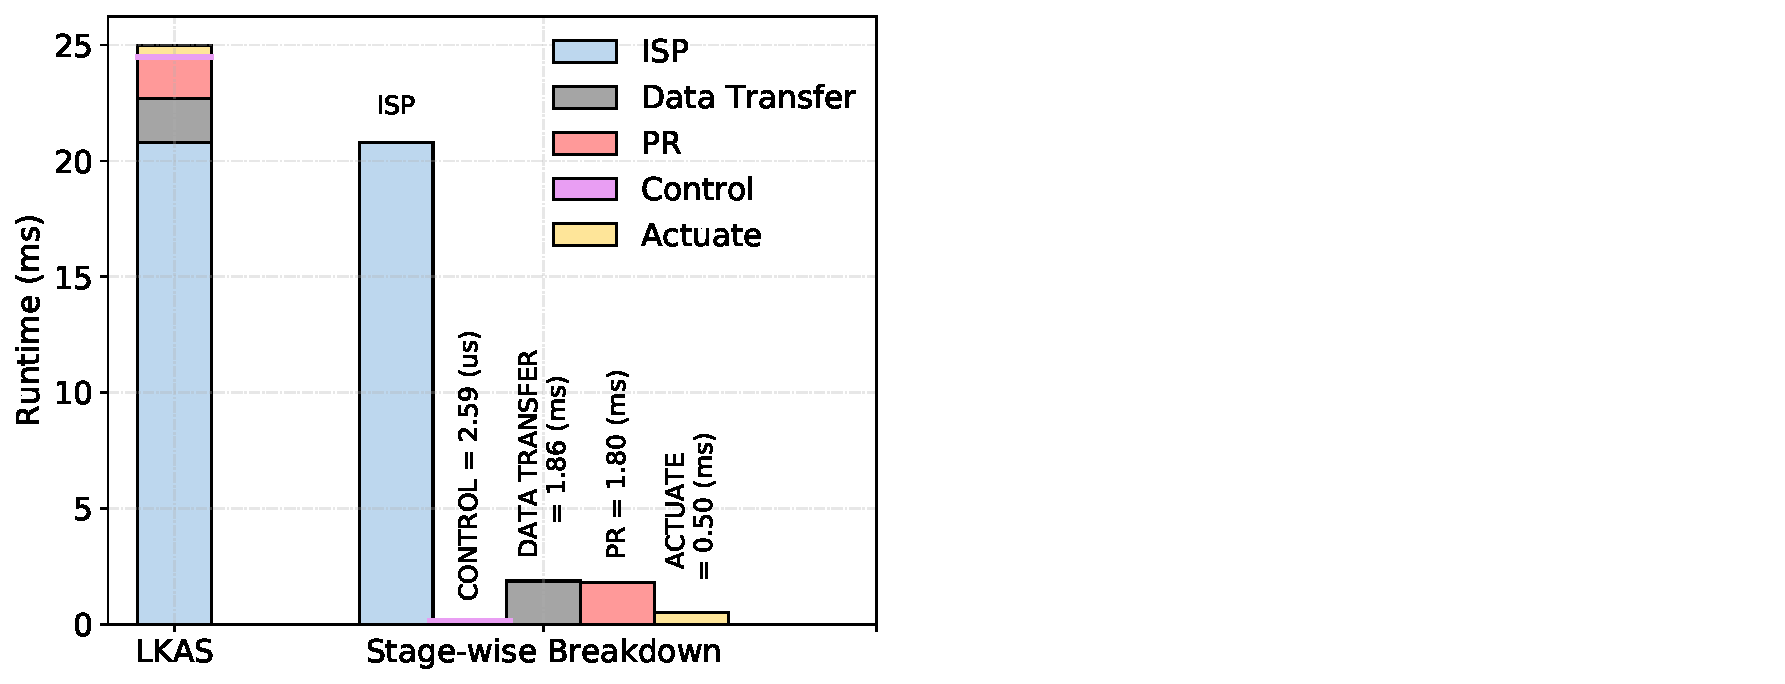
\includegraphics[width= 0.6\textwidth]{figs/profiling_lkas_time.pdf}
	\captionsetup{width=0.8\textwidth}
	\caption{{Full system runtime profiling of \gls{lkas} on NVIDIA AGX Xavier with default configuration (CPU\_8C+GPU).}}
	\label{fig:profile_isp}
% 	\vspace{-5pt}
\end{figure}

\subsection{What should we approximate?}\label{profile}
The first challenge is to identify the error-resilient as well as compute-heavy stages in \gls{lkas}. These are target candidates that can give maximum gains. \Gls{lkas} consists of six different stages, starting with the image capture by the camera sensor and ending with the actuation, as shown in Fig.~\ref{fig:hilsetup}. Actuation cannot be approximated as it depends on vehicle dynamics. However, prior literature has shown that the other stages (camera sensor\cite{buckler}, \gls{isp}\cite{nn_invoke}, data compression\cite{araha}, \gls{pr}\cite{sde}, control\cite{araha2}) can be approximated. So, to figure out the best approximation opportunities, we perform runtime profiling of \gls{lkas}. 

\par Runtime profiling results for \gls{lkas} are shown in Fig.~\ref{fig:profile_isp}. Profiling is performed using the default configuration of the NVIDIA AGX Xavier platform (see Fig.~\ref{fig:platform}~(a)). The system is running Ubuntu 18.04. 
For \textbf{runtime profiling}, we execute each stage in \gls{lkas} 100 times and for 100 different images to reduce sensitivity to access locality. For each stage, we consider the maximum of all such execution runs to get the \gls{wcet}. For actuation, a \gls{wcet} of 0.5 ms is considered \cite{RandyFrank2016}. 

\par From Fig.~\ref{fig:profile_isp}, it is evident that \gls{isp}, which consumes 83\% of the total runtime, is the main target candidate for approximation. Additionally, the off-chip data transfer can also be optimized to obtain added gains. So, in the rest of the chapter, we confine our scope to optimizing the \gls{isp} and the off-chip data transfer.

\subsection{How to approximate and optimize \gls{lkas}?}\label{coarse_approx}
In this work, we propose an approximation-aware design approach shown in Fig.~\ref{fig:optim}. Each of the contributions presented in this chapter is marked. 

% \vspace{-12 pt}
\begin{figure}[ht]
	\centering
	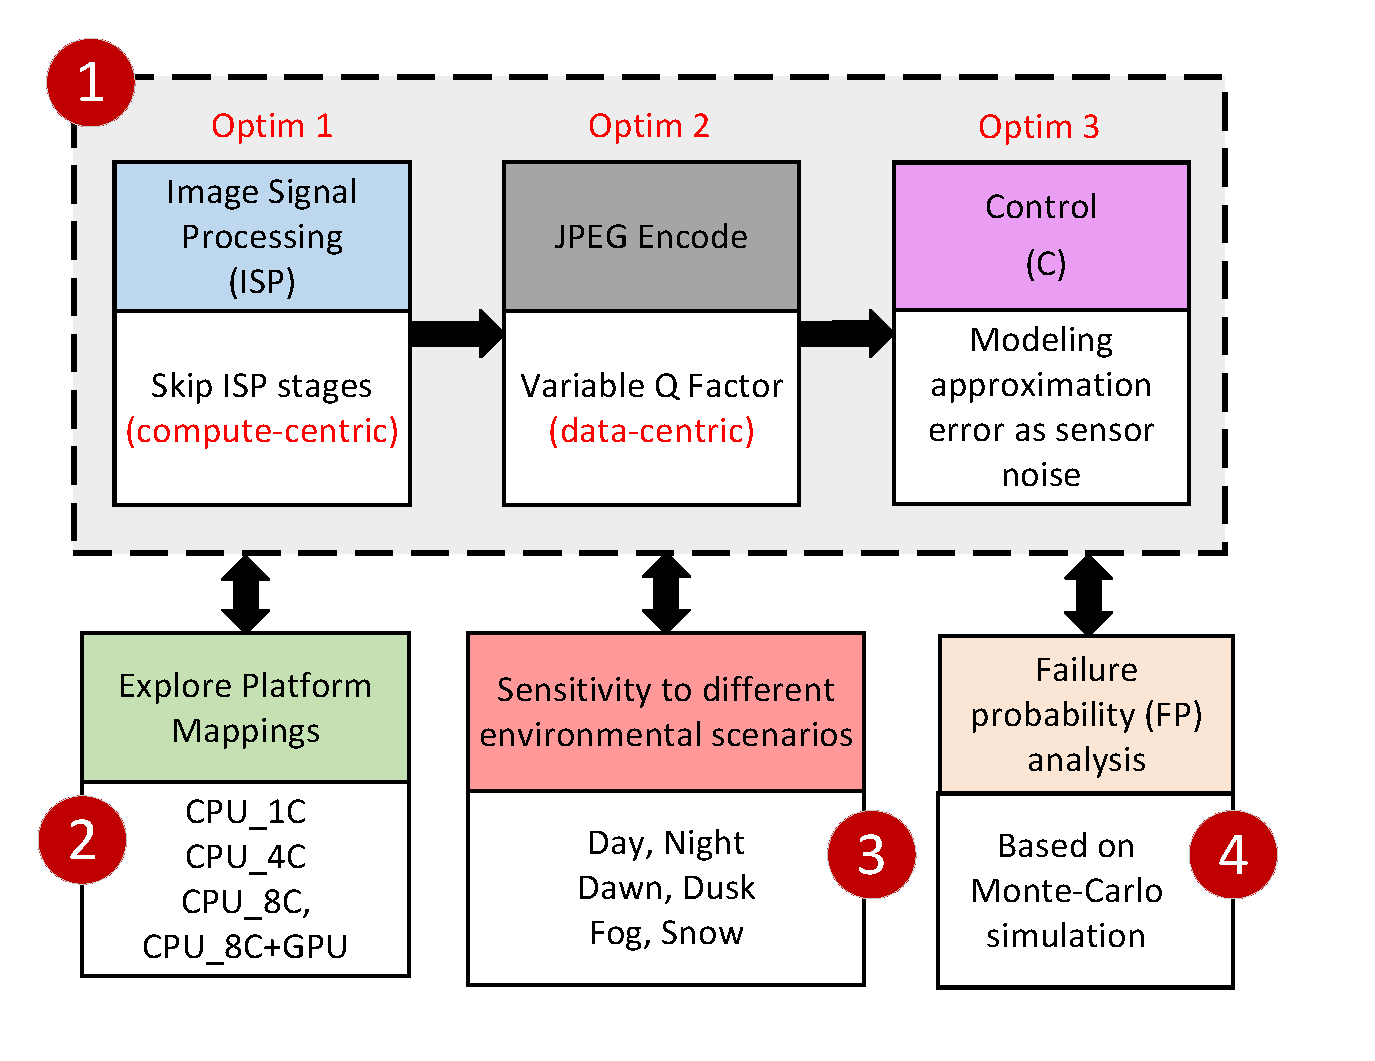
\includegraphics[width= 0.8\textwidth]{figs/optim1_new_v2.pdf}
	\caption{{Proposed approximation-aware design approach for \gls{ibc} systems.}}
	\label{fig:optim}
% 	\vspace{-10 pt}
\end{figure}
\par First, we perform coarse-grained approximations to the \gls{isp} (Optim 1) by skipping one or more sub-stages within the pipeline (see Fig.~\ref{fig:isp}~(a)). This is a compute-centric approximation approach focused on reducing the compute workload of the \gls{isp} \footnote{Note that this compute-centric approach has no impact on the data transfer traffic as the degree of lossy compression performed in the JPEG encoder post-\gls{isp} is fixed to the minimum.}. Then we perform data-centric approximations by varying the degree of lossy JPEG compression (Optim 2). The goal is to reduce the data transfer traffic between the processor and off-chip DRAM, as accessing DRAM is slow. The Q-parameter in the JPEG algorithm decides the degree of lossy compression. A smaller value of Q denotes larger numerical values in the quantization matrix, thereby leading to a higher level of compression. This comes at the cost of larger errors in the decompressed image. In case of Optim 1, we choose the highest value of Q (=100) and keep it constant, which results in a lower degree of lossy compression. However, in the case of Optim 2, we use the Q-parameter as a quality control knob and reduce it in discrete steps of 10 from Q = 100 to Q = 10. This reduces the off-chip data transfer traffic and impacts the \gls{qoc}, and memory footprint of \gls{lkas}. 

\par From a control-design perspective, approximations performed in Optim 1 and Optim 2 introduce errors in the state of the system. The controller is unaware of this added error. So, we design an approximation-aware \gls{lqg} controller (Optim 3) by modelling the error as sensor noise. Profiling results in Fig.~\ref{fig:profile_isp} show that \gls{lkas} is compute-bound. So, we expect most gains from Optim 1 as it reduces the compute workload of the system.  We start by evaluating Optim 1. Then we incrementally add Optim 2 and Optim 3. It is worth mentioning that Optim 1 and 2 are not novel approximation strategies. However, the focus of this work is to evaluate the combined impact of these optimizations (Optim 1, Optim 2, and Optim 3) on the closed-loop \gls{qoc} and memory of the \gls{lkas}, which is not explored in prior literature.

\par \Gls{lkas} operates under different environmental scenarios. We design approximation-aware controllers for each scenario and evaluate the sensitivity of \gls{lkas} to Optim 1, Optim 2, and Optim 3 when operated under these scenarios. We set up six different environmental scenarios (day, night, dawn, dusk, fog and snow) in Webots for analyzing the sensitivity of \gls{lkas} to approximation errors. \gls{lkas} is a safety-critical application that requires an evaluation of its robustness to approximation error. So, we perform a \gls{fp} analysis of approximate \gls{lkas} using \gls{hil} based Monte-Carlo simulation. 
%  \vspace{-10 pt}
\begin{figure}[t]
	\centering
	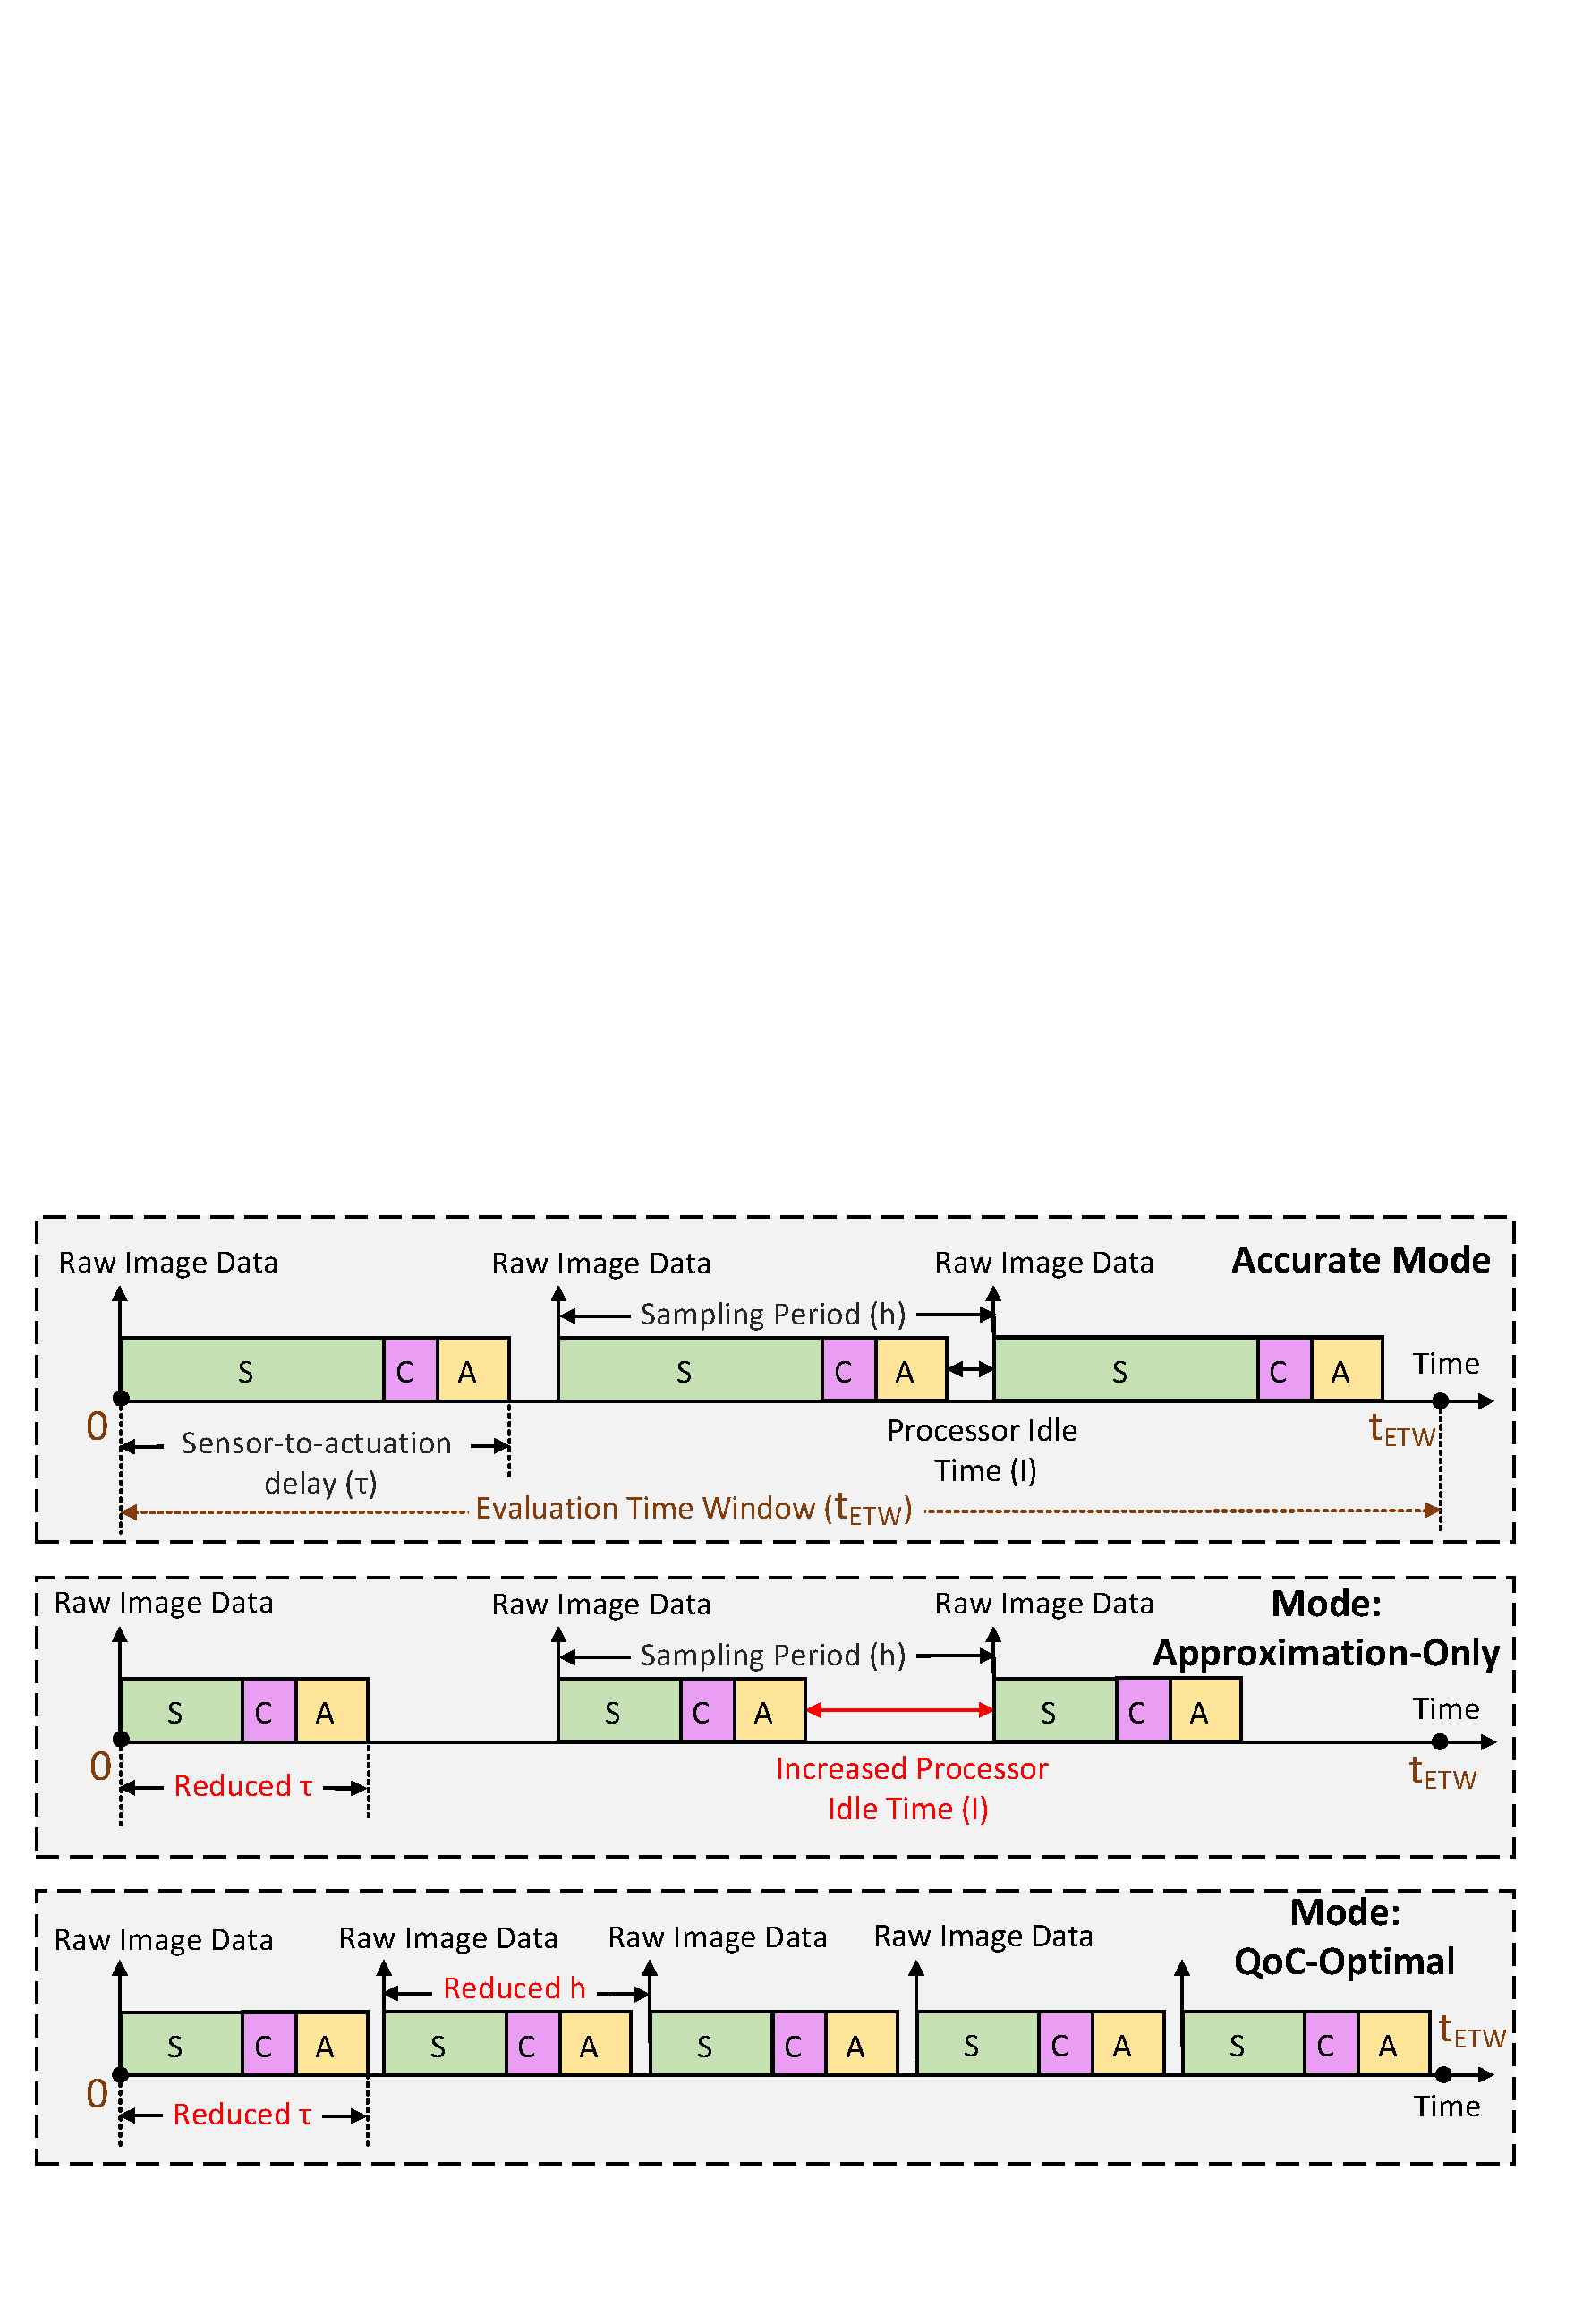
\includegraphics[width= 0.9\textwidth]{figs/modes.pdf}
	%\vspace{-5pt}
	\caption{{Two \gls{lkas} operational modes considered in this work: approximation-only and \gls{qoc}-optimal. The fully accurate mode is shown as a reference to compare the two modes.}}
	\label{fig:modes}
	\vspace{-10pt}
\end{figure}
\subsection{How to analyze approximation-aware design outcomes?}\label{analyze}
To properly analyze the design points obtained from our approximation-aware design approach,  we consider two different modes: \textit{approximation-only} mode and \textit{\gls{qoc}-optimal} mode. Fig.\ \ref{fig:modes} shows a snapshot of \gls{lkas} operating in these modes over a fixed evaluation time window (t$_{ETW}$). In \textit{approximation-only} mode, we consider a reduced sensing-to-actuation delay $\tau$ obtained due to approximations. However, the sampling period $h$ is kept constant.
This mode helps to evaluate the advantage of only the approximation on the \gls{qoc}.
In \textit{\gls{qoc}-optimal} mode, both reduced sensing-to-actuation delay $\tau$ as well as reduced sampling period $h$ are considered. This allows a higher number of frames to be processed over the same t$_{ETW}$.

\subsection{Quality metrics}\label{metrics}
Image quality degradation due to Optim 1 and Optim 2 is evaluated using the \textit{\acrfull{ssim}} index. The  index for two images $m$, $n$ is defined as:
\vspace{5 pt}
\begin{equation} 
%\label{eq2}
\small
SSIM(m, n) = \dfrac{(2\mu_{m}\mu_{n} + C_{1})(2\sigma_{mn} + C_{2})}{(\mu_{m}^2 + \mu_{n}^2 + C_{1})(\sigma_{m}^2 + \sigma_{n}^2 + C_{2})} 
\nonumber
%\vspace{-5 pt}
\end{equation}
\normalsize
\par where $\mu_{m}$, $\mu_{n}$, $\sigma_{m}$, $\sigma_{n}$ and $\sigma_{mn}$ are the local means, standard deviations, and cross-covariance for images $m$, $n$. $C_{1}$, $C_{2}$ are constants. High \gls{ssim} loss denotes images with higher visual difference.
\Gls{qoc} evaluation of the proposed \gls{ibc} system is performed using the metrics \gls{st} (as explained in Section \ref{sec:ch7_QoC_metrics}), \gls{psd}, \gls{mce} (as explained in Section \ref{sec:ch3_control_problem}) and \gls{mae} (as defined below). These metrics consider both control performance and control energy.

  \noindent\textbf{\Acrfull{mae}}: mean of the cumulative sum of absolute errors, i.e.
    %\vspace{-5 pt}
    \begin{equation} 
%    \label{eq1}
    \small
    MAE = \dfrac{1}{n}\sum_{i=1}^{n} |y[k] - \controlRef|
   \nonumber
    %\vspace{-5 pt}
    \end{equation}
    \normalsize
    where $n$ is the no. of samples and $y[k]$ is the value of the $k^{th}$ output. A lower \gls{mae} implies a better \gls{qoc}.

For all evaluations, we consider the following as defaults, unless otherwise mentioned: 
(a) Platform Config: CPU\_8C + GPU (see Fig. \ref{fig:platform} (a)) (b) Scenario: day.